%%%%%%%%%%%%%%%%%%%%%%%%%%%%%%%%%%%%%%%%%
% Article EcoFoG
% Version 2.1 (23/10/2017)
%
% adapté de :
% Stylish Article
% LaTeX Template
% Version 1.0 (31/1/13)
%
% This template has been downloaded from:
% http://www.LaTeXTemplates.com
%
% Original author:
% Mathias Legrand (legrand.mathias@gmail.com)
%
% License:
% CC BY-NC-SA 3.0 (http://creativecommons.org/licenses/by-nc-sa/3.0/)
%
%%%%%%%%%%%%%%%%%%%%%%%%%%%%%%%%%%%%%%%%%


%----------------------------------------------------------------------------------------
%	PACKAGES AND OTHER DOCUMENT CONFIGURATIONS
%----------------------------------------------------------------------------------------

\documentclass[fleqn,10pt]{ArtEcoFoG} % Document font size and equations flushed left

\setcounter{tocdepth}{3} % Show only three levels in the table of contents section: sections, subsections and subsubsections


% Pandoc environments
\usepackage{framed}
\usepackage{fancyvrb}
\providecommand{\tightlist}{%
  \setlength{\itemsep}{0pt}\setlength{\parskip}{0pt}}
\newcommand{\VerbBar}{|}
\newcommand{\VERB}{\Verb[commandchars=\\\{\}]}
\DefineVerbatimEnvironment{Highlighting}{Verbatim}{commandchars=\\\{\}, fontsize=\scriptsize} % Code R
\definecolor{shadecolor}{RGB}{248,248,248}
\newenvironment{Shaded}{\begin{snugshade}}{\end{snugshade}}
\newcommand{\KeywordTok}[1]{\textcolor[rgb]{0.13,0.29,0.53}{\textbf{{#1}}}}
\newcommand{\DataTypeTok}[1]{\textcolor[rgb]{0.13,0.29,0.53}{{#1}}}
\newcommand{\DecValTok}[1]{\textcolor[rgb]{0.00,0.00,0.81}{{#1}}}
\newcommand{\BaseNTok}[1]{\textcolor[rgb]{0.00,0.00,0.81}{{#1}}}
\newcommand{\FloatTok}[1]{\textcolor[rgb]{0.00,0.00,0.81}{{#1}}}
\newcommand{\ConstantTok}[1]{\textcolor[rgb]{0.00,0.00,0.00}{{#1}}}
\newcommand{\CharTok}[1]{\textcolor[rgb]{0.31,0.60,0.02}{{#1}}}
\newcommand{\SpecialCharTok}[1]{\textcolor[rgb]{0.00,0.00,0.00}{{#1}}}
\newcommand{\StringTok}[1]{\textcolor[rgb]{0.31,0.60,0.02}{{#1}}}
\newcommand{\VerbatimStringTok}[1]{\textcolor[rgb]{0.31,0.60,0.02}{{#1}}}
\newcommand{\SpecialStringTok}[1]{\textcolor[rgb]{0.31,0.60,0.02}{{#1}}}
\newcommand{\ImportTok}[1]{{#1}}
\newcommand{\CommentTok}[1]{\textcolor[rgb]{0.56,0.35,0.01}{\textit{{#1}}}}
\newcommand{\DocumentationTok}[1]{\textcolor[rgb]{0.56,0.35,0.01}{\textbf{\textit{{#1}}}}}
\newcommand{\AnnotationTok}[1]{\textcolor[rgb]{0.56,0.35,0.01}{\textbf{\textit{{#1}}}}}
\newcommand{\CommentVarTok}[1]{\textcolor[rgb]{0.56,0.35,0.01}{\textbf{\textit{{#1}}}}}
\newcommand{\OtherTok}[1]{\textcolor[rgb]{0.56,0.35,0.01}{{#1}}}
\newcommand{\FunctionTok}[1]{\textcolor[rgb]{0.00,0.00,0.00}{{#1}}}
\newcommand{\VariableTok}[1]{\textcolor[rgb]{0.00,0.00,0.00}{{#1}}}
\newcommand{\ControlFlowTok}[1]{\textcolor[rgb]{0.13,0.29,0.53}{\textbf{{#1}}}}
\newcommand{\OperatorTok}[1]{\textcolor[rgb]{0.81,0.36,0.00}{\textbf{{#1}}}}
\newcommand{\BuiltInTok}[1]{{#1}}
\newcommand{\ExtensionTok}[1]{{#1}}
\newcommand{\PreprocessorTok}[1]{\textcolor[rgb]{0.56,0.35,0.01}{\textit{{#1}}}}
\newcommand{\AttributeTok}[1]{\textcolor[rgb]{0.77,0.63,0.00}{{#1}}}
\newcommand{\RegionMarkerTok}[1]{{#1}}
\newcommand{\InformationTok}[1]{\textcolor[rgb]{0.56,0.35,0.01}{\textbf{\textit{{#1}}}}}
\newcommand{\WarningTok}[1]{\textcolor[rgb]{0.56,0.35,0.01}{\textbf{\textit{{#1}}}}}
\newcommand{\AlertTok}[1]{\textcolor[rgb]{0.94,0.16,0.16}{{#1}}}
\newcommand{\ErrorTok}[1]{\textcolor[rgb]{0.64,0.00,0.00}{\textbf{{#1}}}}
\newcommand{\NormalTok}[1]{{#1}}
\usepackage{longtable,booktabs}
\usepackage{caption}
% These lines are needed to make table captions work with longtable:
\makeatletter
\def\fnum@table{\tablename~\thetable}
\makeatother
% longtable 2 columns
% https://tex.stackexchange.com/questions/161431/how-to-solve-longtable-is-not-in-1-column-mode-error
\makeatletter
\let\oldlt\longtable
\let\endoldlt\endlongtable
\def\longtable{\@ifnextchar[\longtable@i \longtable@ii}
\def\longtable@i[#1]{\begin{figure}[t]
\onecolumn
\begin{minipage}{0.5\textwidth}\scriptsize
\oldlt[#1]
}
\def\longtable@ii{\begin{figure}[t]
\onecolumn
\begin{minipage}{0.5\textwidth}\scriptsize
\oldlt
}
\def\endlongtable{\endoldlt
\end{minipage}
\twocolumn
\end{figure}}
\makeatother

\usepackage{graphicx,grffile}
\makeatletter
\def\maxwidth{\ifdim\Gin@nat@width>\linewidth\linewidth\else\Gin@nat@width\fi}
\def\maxheight{\ifdim\Gin@nat@height>\textheight0.8\textheight\else\Gin@nat@height\fi}
\makeatother
% Scale images if necessary, so that they will not overflow the page
% margins by default, and it is still possible to overwrite the defaults
% using explicit options in \includegraphics[width, height, ...]{}
\setkeys{Gin}{width=\maxwidth,height=\maxheight,keepaspectratio}

% User-adder preamble
\usepackage{textcomp} \DeclareUnicodeCharacter{B0}{\textdegree}
\usepackage{tabu}
\renewenvironment{table}{\begin{table*}}{\end{table*}\ignorespacesafterend}
\hyphenation{bio-di-ver-si-ty sap-lings}

%----------------------------------------------------------------------------------------
%	ARTICLE INFORMATION
%----------------------------------------------------------------------------------------

\JournalInfo{Hal 00679993} % Journal information
\Archive{DOI xxxx} % Additional notes (e.g. copyright, DOI, review/research article)

\PaperTitle{30 Years of Post-disturbance Recruitment in Tropical Forest} % Article title

\Authors{
Ariane MIRABEL\textsuperscript{1*}\\ Eric MARCON\textsuperscript{1}\\ Bruno HERAULT\textsuperscript{2}
} % Authors
\affiliation{
\textsuperscript{1}UMR EcoFoG, AgroParistech, CNRS, Cirad, INRA, Université des Antilles,
Université de Guyane.\\ \hspace{1em} Campus Agronomique, 97310 Kourou, France.\\\textsuperscript{2}INPHB (Institut National Ploytechnique Félix Houphoüet Boigny)\\ \hspace{1em} Yamoussoukro, Ivory Coast
}
\affiliation{*\textbf{Corresponding author}: ariane.mirabel@ecofog.gf, http://www.ecofog.gf/spip.php?article47} % Corresponding author

\Keywords{Taxonomic and Functional Diversity, Recruitment, Resilience, Tropical Forests, Disturbance Dynamics} % Keywords - if you don't want any simply remove all the text between the curly brackets
\newcommand{\keywordname}{Keywords} % Defines the keywords heading name

%----------------------------------------------------------------------------------------
%	ABSTRACT
%----------------------------------------------------------------------------------------

\Abstract{
The role of trees biodiversity for tropical forests environmental,
economic and social services promt the clarification of its fate in the
global changing climate. Predict the response and resilience of forests
to disturbance requires to understand the processes structuring
communities along time in terms of functioning and taxonomic diversity
and compostition. it would come to Specifically it would come to (i)
disentangle stochastic from determined recruitment underlying
communities and (ii) further specify the deterministic competition rules
involved, and finally (iii) resolve the completeness and duration of
communities resilience. We examined trees diversity and composition
trajectories in a neotropical forest over 30 years after a gradient of
logging and thinning disturbance, by focusing on recruitment processes
that drive communities response to disturbance and determine the various
facets their resilience. Specifically we analysed the trajectories of
three diversities assessing communities taxonomic richness and evennes,
of Rao functional diversity intergrating species ecology through 7 key
functional traits, and of the recruitment taxonomic turnover compared to
pre-disturbance communities. Observed trajectories were besides compared
to null models of stochastic taxonomic and functional recruitment. We
found three-phased recruitment trajectories shaped by a gradual balance
between stochastic and deterministic recruitment. Trajectories first
relied on the stochastic recruitment of pre-disturbance grown saplings,
before the dominance of deterministic recruitment of trees from the seed
bank undergoing competitive exclusion for light. Trajectories eventually
restored the stochastic recruitment specific to old-growth forests along
with communities initial states. Communities resilience was consistent
but while it proved fast in a common functional space among communities
the taxonomic resilience was decades-long and maintained initial
composition differences. The response of tropical forests to disturbance
shaped by deterministic, competitive recruitment ensures taxonomic and
functional resilience. Forests response quickly recovered common
functioning but composition differences, also restored, drove
decades-long recovery diverging among communities. Although promising
for the maintenance of forests' multiple biodiversity facets under a
changing context, these results called cautions regarding the duration
of management practices and the consistency of similar trajectories
after repeted disturbance.
}

%----------------------------------------------------------------------------------------

\begin{document}

\selectlanguage{english}

\flushbottom % Makes all text pages the same height

\maketitle % Print the title and abstract box

\tableofcontents % Print the contents section

\thispagestyle{empty} % Removes page numbering from the first page

%----------------------------------------------------------------------------------------
%	ARTICLE CONTENTS
%----------------------------------------------------------------------------------------


\section{Introduction}\label{introduction}

Determining the response of tropical forests to disturbance is key to
predict their fate in the global changing context. In the last decades,
tropical forests experienced a wide range of disturbance, from radical
land-use changes for agriculture or mining
\citep{Dezecache2017a, Dezecache2017b} to more insidious changes of
communities structure, diversity and functioning following climatic
changes \citep{Aubry-Kientz2015} or anthropogenic activities like
selective logging \citep{Baraloto2012a, Herault2016}. In that respect a
vast literature successfully modeled communities response to disturbance
in terms of tree growth \citep{Gourlet-Fleury2000}, tree height
\citep{Rutishauser2016}, carbon stocks and water and nutrient fluxes
\citep{Putz2012, Martin2015, Piponiot2016}. However, similar approaches
regarding forest diversity remain hindered by the huge biological
diversity constraining studies to focus on common or commercial species,
and by the scarcity of long-term monitoring
\citep{Sebbenn2008, Rozendaal2010, Vinson2015}.

Major insights on forests diversity response to disturbance would be
given by communities trajectories along time. Communities comprise on
the one hand the trees surviving from before disturbance and on the
other hand those recruited afterward \citep{Herault2018}. Surviving
trees already proved mirroring the diversity of pre-disturbance
communities, so communities trajectories and resilience would depend on
the diversity of recruited trees that build the future community. First,
recruitment trajectories depend on the composition and diversity of the
initial, pre-disturbance community that conditions the pool of
recruitable species via the existing saplings and seed bank
\citep{Herault2018}. Then, trajectories depend either on stochastic
recruitment determined by recruitment and dispersal limitations
\citep{Hurtt1995, Hubbell2001}, or deterministic processes like
niche-based competition or biotic interaction \citep{Adler2007}.
Stochastic processes build communities as random samples of the larger
regional-scale forest. Deterministic processes in turn rely at this
spatial scale on the interactions among species and with abiotic
environment that filter-out recruited species following their ecology.
Understand the mechanisms of communities trajectories primarily requires
to estimate the importance of the initial community composition and then
balance between stochastic and deterministic processes. These mechanisms
would then shed light on communities resilience and on the time to
recover pre-disturbance ecosystem properties, eventually to adjust
exploitation and conservation guidelines
\citep{Diaz2005, Gardner2007, Schwartz2017}.

The ecological processes shaping the trajectories differently affect
communities taxonomic characteristics, that consider all species equal,
and functional characteristics, which accounts for species ecology and
functioning \citep{Violle2007b, Kunstler2016}. Two communities may
indeed be very different in terms of species diversity but very similar
in terms of morphological traits and functioning \citep{Villeger2012}.
The differences between taxonomic and functional trajectories are
insightful of recruitment rules, specifically regarding the
deterministic processes and their strengh
\citep{Mayfield2010, Fukami2005}. At this local spatial scale,
deterministic processes rely on competitive interactions among trees
determined by their functional differences in the use of limited shared
resources \citep{Webb2002, Perronne2017}. Determinisitic processes
ruling the assemblages of species are a balance between the differences
in species competitive ability and ecological niche. Differences in
competitive ability will drive the most competitive species to dominance
and the least competitive to elimination, thus decreasing the functional
diversity. Niche differences in turn favor low densities and low
similarity among species, thus increasing the functional diversity
\citep{Ackerly2003, McGill2006, Kunstler2012}. In tropical forests where
the light is limiting, communities response to disturbance proved a
shift from slow-growing, long-lived species with ``conservative''
resource use to fast growing, resource ``acquisitive'' species
\citep{Denslow1980, Molino2001, Bongers2009}.\\
The competition processes at stake would therefore be grasp by key leaf,
wood and life-history functional traits assessing species ecology and
resources acquisition strategy
\citep{Wright2004, Chave2009b, Herault2011, Gerhold2015}.

Beyond the mere understanding of response mechanisms, disentangle
deterministic from stochastic processes insights the underlyings of
communities resilience. Controversies remained about resilience
determinism, entailing the convergence of communities towards a given
structure likely defined by the environment \citep{Clements1916},
opposed to a stochastic point of view entailing commnuities divergence
through species random recruitment \citep{Diamond1975}. Recently both
points of view were reconciled under the hypothesis the communities
diverge in the taxonomic space while they converge in the functional
space with determined diversity and composition in functional niches.
This hypothesis however remains to be tested for in tropical forest,
despite their importance in guiding ecosystems management and
conservation policies.

In this paper we followed the fate of recruited tree communities (60121
individuals) over 30 years on a large disturbance gradient, with 1 to
60\% of forest biomass removed. We assessed the taxonomic and functional
diversity of recruited trees and associated traits trajectories, using a
large functional trait database covering the leaf, wood and life-history
spectra. We besides followed the dissimilarity in composition of
recruited trees compared to the initial communities. Eventually we
compared the observed trajectories to a stochastic recruitment entailing
the recruits random sampling and the randomization of their functional
traits. These trajectories aimed to asses the recruitment mechanisms
underlying forests response to disturbance, specifically assessing (i)
the role of deterministic compared to stochastic processes and (ii) the
competition deterministic processes invovled. Recruitment trajectories
eventually (iii) enlightened the taxonomic and functional facets of
forests resilience and its consequences on forests future.

\section{Material and Methods}\label{material-and-methods}

\subsection{Study Site}\label{study-site}

The Paracou station is located in a lowland tropical rain forest in
French Guiana (5°18'N and 52°53'W). Climate is tropical wet with mean
annual precipitation averaging 2980 mm.y\textsuperscript{-1} (30-y
period) and a 3-months dry season (\textless{} 100
mm.months\textsuperscript{-1}) from mid-August to mid-November, and a
one-month dry season in March \citep{Wagner2011}. Elevation ranges from
5 to 50 m and mean annual temperature is 26°C. Soils are thin acrisols
over a layer of transformed saprolite with low permeability generating
lateral drainage during heavy rains. The disturbance experiment spread
over a network of twelve 6.25ha plots (Table \ref{tab:Tab1}) that
underwent three disturbance treatments in 1986-1987 \citep{Herault2018}.
Dominant families are Fabaceae, Chrysobalanaceae, Lecythidaceae and
Sapotaceae.

\begin{table}

\caption{\label{tab:Tab1}Intervention table, summary of the disturbance intensity for the 4 plot treatments in Paracou.}
\centering
\begin{tabu} to \linewidth {>{\raggedright}X>{\raggedright}X>{\raggedright}X>{\raggedright}X>{\raggedright}X}
\toprule
Treatment & Timber & Thinning & Fuelwood & \%AGB lost\\
\midrule
Control &  &  &  & 0\\
T1 & DBH $\geq$ 50 cm, commercial species, $\approx$ 10 trees/ha &  &  & $[12\%-33\%]$\\
T2 & DBH $\geq$ 50 cm, commercial species, $\approx$ 10 trees/ha & DBH $\geq$ 40 cm, non-valuable species, $\approx$ 30 trees/ha &  & $[33\%-56\%]$\\
T3 & DBH $\geq$ 50 cm, commercial species, $\approx$ 10 trees/ha & DBH $\geq$ 50 cm, non-valuable species, $\approx$ 15 trees/ha & 40 cm $\leq$ DBH $\leq$ 50 cm, non-valuable species, $\approx$ 15 trees/ha & $[35\%-56\%]$\\
\bottomrule
\end{tabu}
\end{table}

\subsection{Inventories Protocol and Dataset
Collection}\label{inventories-protocol-and-dataset-collection}

All trees above 10 cm DBH were mapped and measured annually since 1984.
During inventories, trees were first identified with a vernacular name
assigned by the field team, and afterward with a scientific name
assigned by a botanist during regular botanical campaigns. Botanical
campaigns have been carried out every 5 to 6 years from 2003 onwards.
These changes in identification protocol raised methodological issues as
vernacular names usually correspond to different botanical species,
resulting in significant taxonomic uncertainties that were propagated to
composition and diversity metrics. Vernacular names were replaced
through multinomial trials
\(M_v\Big(\big[s_1, s_2, …, s_N\big],\big[\alpha_1, \alpha_2,…, \alpha_3\big]\Big)\)
based on the observed association probability
\(\big[\alpha_1, \alpha_2,…, \alpha_3\big]\) between each vernacular
name \emph{v} and the species \(\big[s_1, s_2, …, s_N\big]\) recorded in
the inventory. See appendix 1 and \citet{Aubry-Kientz2013} for the
detailed methodology. To avoid remaining identification caveats, the
simulated botanical inventories were reported at genus level.

Eight functional traits were considered, representing leaf economics
(leaves thickness, toughness, total chlorophyll content and specific
leaf area), wood economics (wood specific gravity and bark thickness)
and life history traits (maximum specific height and seed mass). Traits
were exctracted from the BRIDGE project \footnote{http://www.ecofog.gf/Bridge/}
where trait values were measured on nine forest plots infrench guianan,
including two in Paracou. Missing trait values of the trait database
(10\%) were filled by multivariate imputation by chained equation using
the Mice r package \citep{Mice2011}. As traits variability was lower
within genus and families, we accounted for the phylogenetic signal of
the functional traits by restricting the gap filling processes to
samples pertaining to the next higher taxonomic level. As seed mass
information corresponded to a classification into discrete mass classes,
no data filling process was applied so analysis were performed only
considering the 414 botanical species of the seed mass dataset.

\subsection{Recruitment trajectories}\label{recruitment-trajectories}

To disentangle the recruitment processes from overall dynamics,
communities were split into per-disturbance surviving trees and those
recruited since disturbance. Recruited communities were examined either
considering the ``punctual recruitment'', \emph{i.e.} recruited trees by
2-year intervals, or all recruits since disturbance as the ``accumulated
recruits''. Eventually, in disturbed plots the recruited communities
were examined distinguishing the undisturbed and logging gap areas to
test the validity of recruitment processes for the whole area.

The taxonomic diversity was assessed through Richness and the Hill
number translation of Shannon and Simpson indices
\citep{Hill1973, chao2015estimating, Marcon2015b}.\\
The three diversities belong to the set of HCDT or generalized entropy,
respectively corresponding to the 0, 1 and 2 order of diversity
(\emph{q}), which grasps the balance between richness and evenness in
the community through the value of \emph{q} that emphasizes common
species. Functional trajectories were estimated with the Rao quadratic
entropy, a useful summary variable assess both functional richness and
evenness \citep{Clark2012}, measuring the functional divergence within
communities using Gower distance as recommended by \citet{Pavoine2009}.
Functoinal diversity was completed by the trajectories of traits
community weighted means (CWM), representing the average trait value in
a community weighted by relative abundance of the species carrying each
value \citep{Diaz2007, Garnier2004, Mason2013}. Seed mass trajectories
were reported by the proportion of each class recorded in the
inventories. The similarity between the recruited trees and the
pre-disturbance forest was measured with the turnover metrics detailed
in \citet{Podani2013a}. To estimate the importance of stochastic
processes the recruitment was compared to the trajectories of a
stochastic model corresponding to random samplings. For the taxonomic
trajectories the stochastic model was a random sampling of individual
trees according to their observed abundance that preserved species
abundance and tree density. For for the functional diversity the
stochastic model was a shuffling of functional trait values among
species that randomizes abundances across species but within coomunities
\citep{Mason2013}.

All composition and diversity metrics correspond to the median and 90\%
percentile obtained after 50 iterations of the taxonomy uncertainty
propagation framework and the gap filling process. The stochastic
trajectories were similarily obtained after 50 iterations of the random
sampling.

\section{Results}\label{results}

\subsection{Recruitment Diversity}\label{recruitment-diversity}

All the trajectories were identical in disturbed and undisturbed areas,
confirming that recruitment processes applied to whole communities and
were not restricted to logging gaps.

\subsubsection{Taxonomic Diversity}\label{taxonomic-diversity}

The diversity trajecctories of punctual recruitment followed a
consistent trajectory after disturbance, first with an increase of the
richness and a decrease of the evenness (Figure (\ref{fig:DivTraj}). For
all disturbed plots both richness and evenness tended to return towards
initial values but none had recovered 30 years after disturbance. The
accumulated recruits displayed sharp increasing richness (order 0) and
decreasing evenness (order 2) after intense disturbance (T3 and some T2,
Appendix I, fig. S1).

\begin{figure*}

{\centering 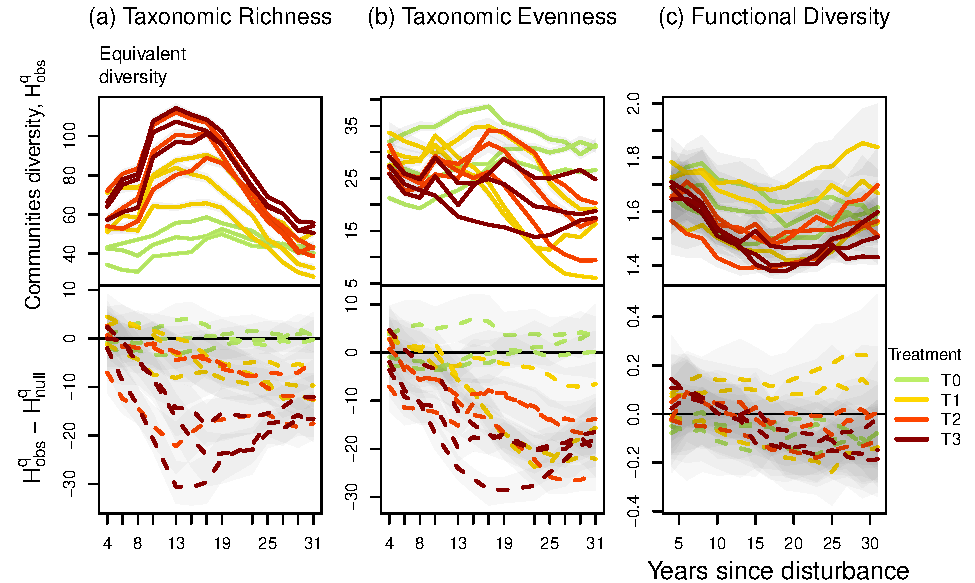
\includegraphics[width=0.8\linewidth]{RecruitmentTrajectories_files/figure-latex/DivTraj-1} 

}

\caption{Trajectories of Richness, Shannon and Simpson diversity for 2-years laps punctual  recruitment (upper panels) and divergence to null model (lower panels). Lines colors refer to the perturbation regime: green for control, blue for T1, orange for T2 and red for T3 disturbance treatments. Plain lines correspond to the median observed after uncertainty propagation and are given along with the 95\% confidence interval (grey envelope).}\label{fig:DivTraj}
\end{figure*}

Punctual and accumulated recruitment diversities were then compared to
the stochastic trajectories of a random sampling. Richness (order 0) and
evenness (order 2) of punctual recruits remained equivalent or higher
than for a random sampling in control plots while both were lower in
disturbed plots. Disturbed plots however followed humped-shaped
trajectories heading towards a recovery of the initial state (Figure
\ref{fig:DivTraj}). Accumulated recruitment richness and evenness were
higher or equivalent to those of the random sampling after low
disturbance intensity (plots T1 and some plots T2) but lower after
intense disturbance (plots T3 and a plot T2, Appendix I fig. S1).

\subsubsection{Functional Diversity and
Composition}\label{functional-diversity-and-composition}

Communities functional diversity was measured with the Rao diversity and
compared to the stochastic trajectories of a random traits shuffling. In
disturbed plots (T2 and T3), the functional diversity decreased until 15
years after disturbance (Figure \ref{fig:FunTraj}) before recovering
towards the initial values. While the recovery was not achieved for the
most disturbed plots, the functional diversity of lighter disturbance
plots recovered faster and for some T1 plots exceeded the initial
values. For all plots, disturbed or not, the observed functional
diversity was lower than this of the random model, to the exception of
two plots T1.

\begin{figure}

{\centering 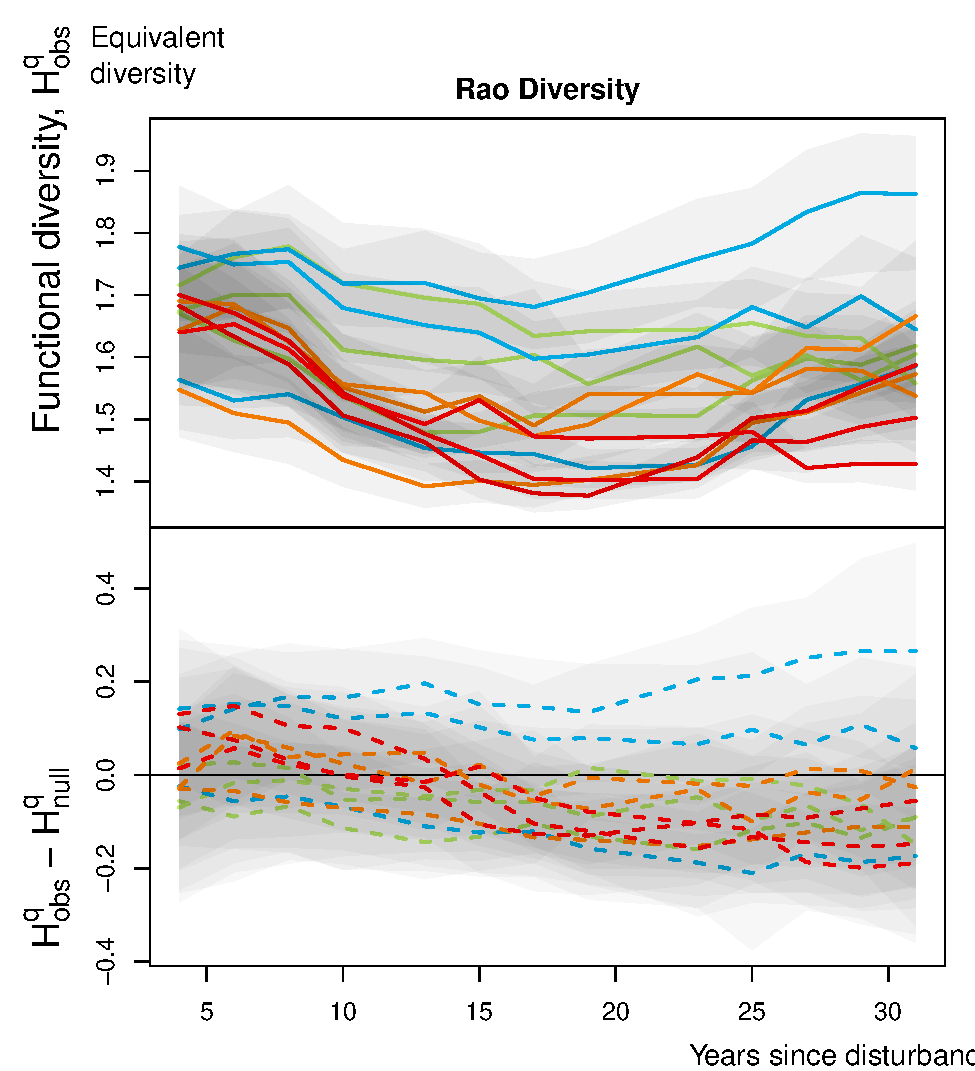
\includegraphics{RecruitmentTrajectories_files/figure-latex/FunTraj-1} 

}

\caption{Functional diversity of punctual recruited trees from the considered functional traits and divergence to null model. Values reported correspond to the plot-level median and the 95\% confidence interval obtained after 50 repetition of the taxonomic uncertainty propagation and the functional database gap-filling processes and 50 run of the null model. Lines colors correspond to the logging treatment initially applied (green for control, blue for T1,orange for T2 and red for T3).}\label{fig:FunTraj}
\end{figure}

Trajectories of the functional traits showed a switch in disturbed plots
towards species with large exchange surface area, light tissues (high
SLA, low leaf toughness and thickness and low wood specific gravity)
with smaller maximum height (Figure \ref{fig:CWM}). Functional traits
either followed hump-shaped trajectories with an ongoing recovery or an
achieved return to the initial state (for SLA,Bark thickness and leaf
thickness and Hmax to a certain extent).

\begin{figure*}

{\centering 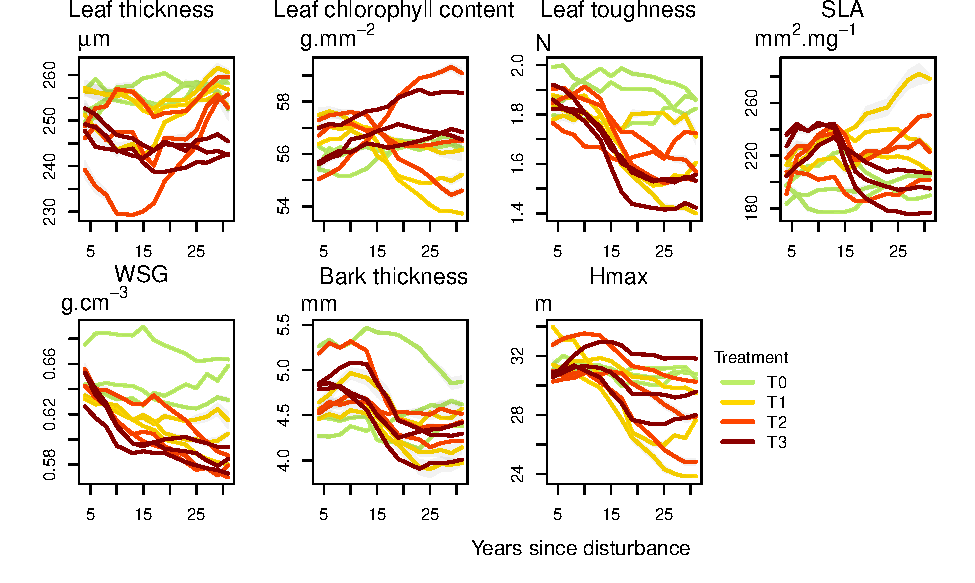
\includegraphics[width=0.8\linewidth]{RecruitmentTrajectories_files/figure-latex/CWM-1} 

}

\caption{Community weighted means (CWM) of the four disturbance treatment for the four leaf traits, the two stem traits  and the specific Hmax. Values reported correspond to the plot-level median obtained after 50 repetition of the taxonomic uncertainty propagation and the functional database gap-filling processes. Lines colors correspond to the disturbance intensity (green for control, blue for T1,orange for T2 and red for T3).}\label{fig:CWM}
\end{figure*}

\subsection{Recruitment Turnover}\label{recruitment-turnover}

In control plots species turnover remained highly stable for the 30
sampled years (Figure \ref{fig:Turnover}), reflecting a strong
similarity between the initial plots composition and the punctual
recruits. In disturbed plots, the taxonomic turnover followed a marked
hump-backed trajectory, with a maximum value reached around 15 years
after disturbance and a maximum positively correlated to the disturbance
intensity (\(\rho_{spearman}=0.93\)). Thirty years after disturbance the
turnover of all disturbed plots had return to low values close to zero.

\begin{figure}

{\centering 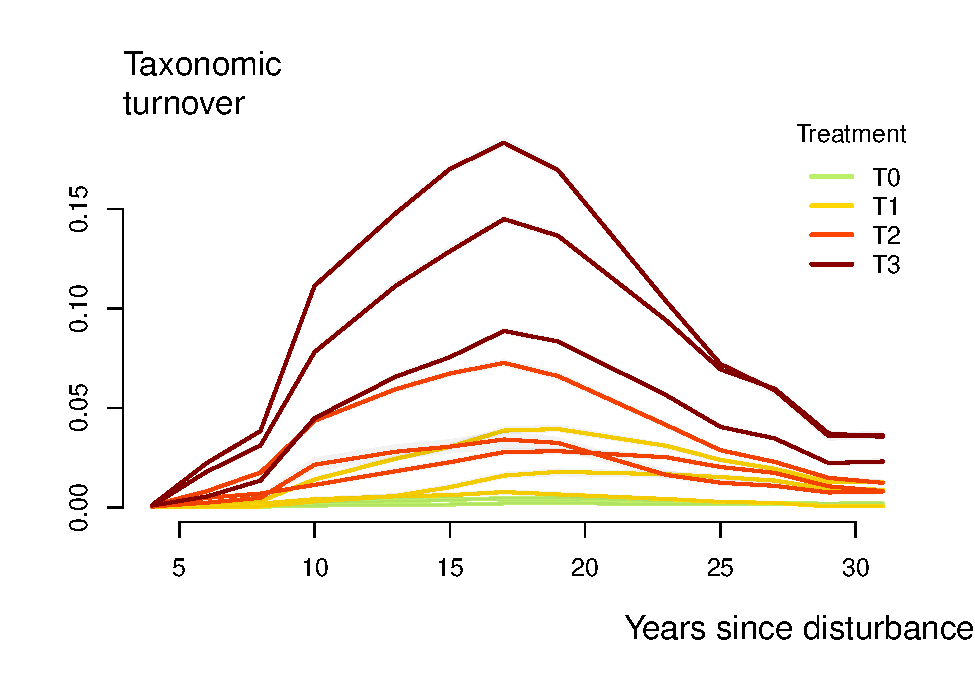
\includegraphics{RecruitmentTrajectories_files/figure-latex/Turnover-1} 

}

\caption{Trajectories over the 30 sampled years of the abundance-based turnover between recruited trees and intial communities before disturbance. Grey envelopes correspond to the 0.025 and 0.975 percentiles of the uncertainty propagation procedue and lines to the median in green for control, blue for T1,orange for T2 and red for T3).}\label{fig:Turnover}
\end{figure}

\section{Discussion}\label{discussion}

\subsection{The three phases of recruitment
trajectories}\label{the-three-phases-of-recruitment-trajectories}

Along the 30 years, the recruitment richness and species turnover
compared to the initial composition, and the trajectories of key
functional traits (SLA and bark thickness) exhibited clear hump-shaped
trajectories, revealing three distinct recruitment phases. Communities
trajectories involved an interplay between stochastic and deterministic
recruitment, first involving species competitive exclusion and then
niche partitioning, before recovering initial recruitment processes.

As a first step (0-8 years), recruited trees showed low turnover
compared to the initial composition and matched the functional diversity
of a stochastic recruitment process. This first recruitment phase
mirroring the old-growth pre-disturbance community then likely involved
already grown saplings (DBH \textless{}10cm) immediatly benefitting from
the increased enlightment and the alleviated competition induced by
disturbance \citep{Herault2010}.

A second phase (8-15 years) then fall into place, corresponding to
marked changes in several functional traits trajectories and to a
decrease in recruitment evenness and functional diversity. This second
phase likely incorporated true recruits, \emph{i.e.} trees germinated
from the seed bank that constitute the main part of the recruitment
\citep{Lawton1988}. The pool of species recruited then was restricted
according to their resource acquisition strategy and revealed the
deterministic processes that balanced the stochastic recruitment
observed in the first place. Indeed, sharp changes in the SLA, wood
density and leaf thickness trajectories occured after intense
disturbance and revealed the prominent recruitment of short-lived, fast
growing hard pionneer species with competitive and efficient light
acquisition \citep{Wright2004, Chave2009b, Herault2011, Reich2014}.\\
The recruitment was therefore shaped by exclusive competition among
species based on their competitive ability differences for light
acquisition \citep{Mayfield2010}, as already demonstrated in for tree
species in temperate forests \citep{Kunstler2012}. The balance between
deterministic and stochastic processes shaping the second phase was
determined by the initial disturbance intensity. After light disturbance
(T1 plots), despite the pool of recruited species was restricted, the
species turnover compared to initial state remained low. Recruited trees
then still mirrored the pre-disturbance communities but recruited
species were more pioneers and light demanders, with strategies of
efficient resource acquisition (high SLA and leaf chlorophyll content)
and inexpensive, short-lived tissues (low leaf thickness and thoughness,
small Hmax and low wood density and bark thickness)
\citep{Hubbell1999, Schnitzer2001, Sheil2003, Bongers2009}. At this
disturbance intensity the recruitment evenness and functional diversity
remained high so despite the selection of more light-demanding species
the recruitment was not overwhelmed by hard pioneers. This might be
explained by the recruitment and dispersal limitations due to the short
dispersal distance observed for tropical trees, specifically in Paracou
with the genetic clumping of some pioneers
\citep{Leclerc2015, Scotti2015a}. After intense disturbance in contrast
(T2 and T3 plots), the recruitment rapidly differed from the
pre-disturbance composition and corresponded to a sharp increase of the
SLA and bark thickness. These drastic trajectories changes reflected an
overhelming recruitment of hard pioneers likely entailing significant
changes in communities functioning \citep{Diaz2005}.

A third recruitment phase eventually entailed a return towards initial
taxonomic and functional diversities. Recruited species remained mainly
light-demanding and still submitted to competitive exclusion, but their
functional diversity and their compositional similarity with initial
communities progressively increased which revealed the recovery of
stochastic recruitment processes dominating in mature forests
\citep{Lawton1988, Mayfield2010}.

The recruitment trajectories proved identical in disturbed versus
untouched areas with plots, suggesting community scale processes. In
undisturbed forests the light availability proved quite homogeneous and
unrelated to trees recruitment success \citep{Dalling2002} while
disturbance gaps and associated edge effect significantly increasing the
global enlightment enhancing trees recruitment success
\citep{Ruger2009}.

\subsection{The questioned completeness of communities
resilience}\label{the-questioned-completeness-of-communities-resilience}

After 30 years, although taxonomic and functional diversity had
recovered initial values, the recruitment processes remained constrained
by the deterministic selection of recruited species contrasting with the
stochastic recruitment of undisturbed forests. The recruitment processes
proved then consistently resilient but over long time period.

The recovery of both recruitment processes and initial composition and
diversity meant the maintenance of pre-disturbance differences in
communities taxonomy. This entailed the existence of multiple stable
equilibrium among communities, corresponded to the initial commmunities
restored after disturbance, consistently with the assumptions made for
highly diverse and productive ecosystems \citep{Chase2003}. Besides it
meant the dependence of communities response on their initial
composition that oriented their trajectories, consistently with previous
observation and with the involvement of pre-disturbance grown saplings
and local seed bank \citep{Dalling2002, Anderson2007}.

In contrast the trajectories of some traits and of functional diversity
were essentially similar among treatments and recovered quickly. This
translated the confluence of communities in the functional space quickly
resotring communities functioning, despite their divergence in the
taxonomic space \citep{Fukami2005}. This confirmed previous results from
the Paracou experiment, conducted 10 years \citep{Molino2001} and 20
years \citep{Baraloto2012a} after disturbance, where the early signs of
the resilience of taxonomic and functional composition had been
detected.

Although consistent communities recovery proved slow, specifically for
taxonomic diversity and several functional traits that remained altered
30 years after disturbance. The disturbance response besides impacted
the seed bank, that is the stock of recruitable species and that
determines communities recoveryresilience. Its involvment might
therefore alter the resilience and future trajectories of communities
\citep{Norden2009}.

\section{Conclusion}\label{conclusion}

The hindsight of the 30 years of forest monitoring highlighted a
three-phase disturbance response, defined by the balance between
stochastic and determinisitic recruitment processes. Communities
trajectories were first driven by the stochastic recruitment of
already-grown saplings mirroring the pre-disturbance state before it was
shaped by the true recruits from the seed bank that underwent
competitive exclusion based on species light acquisition strategy. After
intense disturbance the second recruitment phase was dominated by
short-lived hard pioneers that drastically changed the diversity and the
functioning of communities. A third phase eventually carried out the
recovery towards the initial communities with the resurgence of
stochastic recruitment progressively balancing the competitive exclusion
for resources. The recruitment response to disturbance demonstrated
communities quick functional resilience in a common functional space
while it highlighted the long-term taxonomic resilience, \emph{i.e.}
several decades, that maintained initial composition differences. Even
though the accurate impact on the seed bank remains to be clarified,
communities recovery was tangible but its length entailed great caution
regarding forests management guidelines that aim to a complete recovery
of ecosystems.

\begin{center}\rule{0.5\linewidth}{\linethickness}\end{center}

%----------------------------------------------------------------------------------------
%	REFERENCE LIST
%----------------------------------------------------------------------------------------

\bibliographystyle{mee}
\makeatletter
% The filename has .bib extension the must be eliminated
\filename@parse{references.bib}
% parse stores the file name in base. Extension starts at the first dot, so don't use dots in file names.
\bibliography{\filename@base}
\makeatother


%----------------------------------------------------------------------------------------

\end{document}
